\documentclass[11pt,twoside,openright]{report}
\usepackage{standalone}
\standalonetrue
\ifstandalone
  \usepackage{../../haziq_thesis}  
  \usepackage{../../haziq_maths}
  \usepackage{../../haziq_glossary}
  \usepackage{../../knitr}
  \addbibresource{../../bib/haziq.bib}
  \externaldocument{../../.texpadtmp/phd-thesis}
\fi

\begin{document}
\hChapterStandalone[6]{Bayesian variable selection using I-priors}
\thispagestyle{chaptersix}
\hsetpagenumstandalone{chapter6}

\index{linear regression}
Earlier in \cref{sec:various-regression} \colp{\mypageref{sec:various-regression}}, we saw that model \cref{eq:model1} subject to normal assumptions \cref{eq:model1ass}, model assumptions \ref{ass:A1}--\ref{ass:A3}, and $f$ belonging to the canonical RKHS of functions over $\cX \equiv \bbR^p$ yields the standard multiple regression model
\begin{align}\label{eq:linmod}
  \begin{gathered}
    y_i = \alpha + \sum_{k=1}^p x_{ik}\beta_k + \epsilon_i \\
    \epsilon_i \iid \N_n(0, \sigma^2).
  \end{gathered}  
\end{align}
In this chapter, we use the notation $\sigma^2 = \psi^{-1}$ to denote the error variance.
Furthermore, an I-prior on the regression coefficient entails prescribing the following normal prior the $\beta_k$'s:
\[
  \bbeta := (\beta_1,\dots,\beta_p)^\top \sim \N_p (\bzero,  \kappa \sigma^2 \XTX).
\]
This follows from \cref{eq:ipriorcanonical} after a slight reparameterisation of the RKHS scale parameter $\kappa \mapsto \lambda^2/\sigma^4$. 
Throughout this chapter, we assume that the columns of the design matrix $\bX = (X_1,\dots,X_p)$ have been standardised, so that a single RKHS scale parameter is sufficient for the $p$ covariates.

The topic of interest for this chapter is model selection for linear regression models.
That is, from a set of $p$ covariates or predictors $\{X_1,\dots,X_p\}$, the task is to determine the best choice of subset(s) of variables that should be included in a regression model used to explain the variation in the response variable.
As such, the term \emph{variable selection} is synonymous to model selection for linear regression models.
Fundamental to this notion of variable selection is an inherent belief in sparseness of the true data generative process surrounding the response variable, i.e. not all of the variables need be used to predict the response.
Model selection is indeed a huge topic to cover fully.
We broadly classify variable selection into three categories: 1) (pairwise) model comparison using some criterion; 2) shrinkage to induce sparsity; and 3) Bayesian model selection.
We understand that different categorisations and hence categories of model selection exist in the literature, but our focus is on the discussion of the three types as mentioned.

\index{model selection}
Model selection criteria, both from a frequentist and Bayesian standpoint, can either be of a predictive nature (e.g.  $R^2$, mean squared error of prediction (MSEP), $C_p$ \citep{mallows1973some}, $k$-fold cross-validation MSEP, etc.), or based on likelihood (e.g. likelihood ratios, Bayes factors, Akaike information criterion (AIC, \cite{akaike1973}), Bayesian information criterion (BIC, \cite{schwarz1978estimating}), etc.).
Selecting a model based on either of these criteria requires comparison of all $2^p$ criteria, which is not feasible for large $p$.
Typically, these criteria are used in conjunction with stepwise procedures such as forward-selection or backward-deletion to restrict attention to a smaller number of potential subsets \citep{George1993,miller2002subset}.

\index{regularisation}
\index{Lasso}
\index{ridge regression}
On the other hand, regularised least squares regression (ridge regression \citep{hoerl1970ridge}, Lasso \citep{tibshirani1996regression}, or a convex combination of the two via elastic nets \citep{zou2005regularization}, etc.) provide additional information to the regression model in order to provide a sparse solution to linear system of equations in $\bbeta$.
These methods are proven to be popular as they are fast and perform exceptionally well in many situations, even in cases where $p > n$.
Additionally, the Lasso produces solutions for $\bbeta$ which are exactly zero.
However, the Lasso in general produces estimates which are biased towards zero, are inconsistent, and have no valid standard errors \citep{friedman2001elements,kyung2010penalized}.
Further criticisms of the Lasso include its inability to select more than $n$ predictors in a $p>n$ situation, and poor performance when multicollinearity exists among the covariates.

From a Bayesian perspective, regularisation is akin to placing priors on the $\beta_k$'s to shrink the effects of the $\beta_k$'s: the ridge regression has a Bayesian interpretation of placing normal priors on the regression coefficients, while the Lasso a Laplace or double exponential prior \citep{park2008bayesian}.
The term adaptive shrinkage has been used for the method in which hyperpriors are placed on the scale parameter of the prior for the $\beta_k$'s.
The idea is to adaptively shape the prior depending on the importance of the variable in the regression model.
Bayesian shrinkage includes the task of specifying tuning parameters, which could potentially affect chain mixing in a Markov chain Monte Carlo method (MCMC) procedure, which is the estimation method that is commonly used.

\index{Bayesian model selection}
True Bayesian model selection is probabilistic in nature: a priori, one assigns probabilities over the set of models, and then after observing the data, posterior model probabilities (PMPs) are used to discern which of the models was likeliest to have been behind the data generative process of the observed responses.
Of course, with large  $p$, calculation of all $2^p$ posterior model probabilities to ascertain which is highest will be a challenge, if not impossible.
But, as with most Bayesian applications, MCMC can be applied as a practical means of overcoming this intractability.
This stochastic approach to variable selection was pioneered by \citet{George1993}, and studied by others such as \citet{Kuo1998,dellaportas2002bayesian,Ntzoufras2008}.
Unlike shrinkage methods, Bayesian model selection is able to quantify the amount of times a variable ``enters the model'' (inclusion probabilities), and thereby measuring its worth as a  predictor.

\thispagestyle{chaptersix}
\index{Bayesian model averaging}
Note that, in addition to model probabilities and inclusion probabilities, estimates of regression coefficients are obtained simultaneously in Bayesian variable selection.
When several competing models have high posterior probabilities, regression coefficients from each model, or indeed any quantity of interest, may be combined and weighted using their posterior model probabilities, a technique known as \emph{Bayesian model averaging} \citep{madigan1994model,hoeting1999bayesian}.
Averaging over a set of models takes into account the uncertainty surrounding model selection, which other standard statistical procedures ignore upon selection of a single model from which to do inference.
It is known to be the case that predictive accuracy of the model-averaged quantity is improved, as measured by a logarithmic scoring rule \citep{raftery1997bayesian}.

\label{errata18}
Bayesian model selection is not without criticism, however.
For complex models with many predictors or samples, MCMC is slow and may mix poorly \citep{OHara2009}.
Often, there are a lot of tuning parameters that need to be set correctly for the problem at hand.
Also, the choice of priors for model parameters affects consistency of Bayesian model selection procedures. 
Specifically, improper priors cannot be used to calculate posterior model probabilities \citep{casella2009consistency}---otherwise, one risks running into Lindley's paradox\footnote{Briefly, in testing a point null hypothesis of the mean of a normally distributed parameter, the null hypothesis is increasingly accepted as the prior variance of the parameter approaches infinity, regardless of evidence for or against the null.
The paradox is also termed Jeffreys-Lindley paradox \citep{robert2014jeffreys}.} \citep{lindley1957statistical}.

The plan for this chapter is to describe a fully Bayesian model for variable selection using I-priors. 
The approach that we take is a stochastic search of the model space due to \citet{Kuo1998}, realised through a simple Gibbs sampling procedure.
The main motivation behind using I-priors in Bayesian variable selection is its suitability in accommodating to datasets with strong multicollinearity and being able to run with little to no prior information about the parameters.
A simulation study is conducted and several real-world examples presented to demonstrate this fact. 

\section{Preliminary: model probabilities, model evidence and Bayes factors}

The paradigm of model selection is as follows. 
From a finite set of models $\cM = \{M_1,\dots,M_K\}$, pairs of data $\{(y_1,\bx_1),\dots,(y_n,\bx_n)\}$, $y_i\in\bbR$ and $\bx_i\in\cX\equiv\bbR^p$, had been generated according to the generative process dictated by one of the models $M_k \in \cM$ and its respective parameters $\Theta_k$.
Having observed only this data set, the goal is to infer which of the models had generated the data, and consequently obtain estimates for the parameters.
It is perhaps most natural to ponder which of the models is most likely to be the ``true'' one given the data presented, and thus, this natural way of thinking leads one to the concept of \emph{model probabilities}.
From a Bayesian perspective in particular, \emph{posterior model probabilities} allow us to quantify the certainty to which any model is behind the data generative process, after taking into account relevant evidence (observation of the data) and prior beliefs about model and parameter uncertainty.
\index{model probabilities}

Let $p(M_1),\dots,p(M_K)$ be prior probabilities assigned to the model space $\cM$, and $p(\Theta_k|M_k)$ be the prior on the parameters of model $M_k$.
For any model $M_k \in \cM$, the posterior model probability for model $m$ is
\begin{align}\label{eq:pmp}
  p(M_k|\by) 
  &=\frac{p(\by|M_k)p(M_k)}{\sum_{k=1}^K p(\by|M_k)p(M_k) } 
\end{align}
where 
\begin{align}\label{eq:modelevidence2}
  p(\by|M_k)
  &= \int p(\by|M_k,\Theta_k)p(\Theta_k|M_k) \dint\Theta_k
\end{align}
is known as the marginal likelihood, or \emph{evidence}, for model $M_k$.
As a remark, the prior distributions for the parameters do not necessarily need to depend on the model, so we might have that $p(\Theta_k|M_k)=p(\Theta_k)$.
A natural strategy for model selection is to select the model such that $p(M_k|\by)$ is largest (the \emph{highest probability model}, HPM), but several models rather than just a single one may be reported to convey model uncertainty \citep{Chipman2001}.
\index{highest probability model}

Note, that models may be pairwise compared based on these posterior model probabilities, for which the posterior odds
\vspace{-0.9em}
\begin{equation}
  \frac{p(M_k|\by)}{p(M_0|\by)} = 
  \myoverbrace{\frac{p(\by|M_k)}{p(\by|M_0)}}{\text{Bayes factor}}
  \times 
  \myoverbrace{\frac{p(M_k)}{p(M_0)}}{\text{prior odds}}
\end{equation}
provide a point summary for comparing model $M_k$ against model $M_0$.
The first term on the right-hand side is the Bayes factor for comparing any model $M_k \in \cM$ to another model $M_0 \in \cM$, and is denoted by $\text{BF}(M_k,M_0)$.
Thus, model selection based on posterior model probabilities can be formalised as the Bayesian alternative to classical hypothesis testing using Bayes factors \citep{kass1995bayes}.
\index{Bayes factor}
\index{Bayesian hypothesis test}

The issue that is faced with Bayesian model selection is that all posterior model probabilities must be calculated in order for a full comparison to be made.
When the model space is very large, this can prove to be an insurmountable task.
In the case of linear regression, where each of the $p$ variables may be selected or not, the size of the model space is $2^p$.
Even for moderate sized $p$ this can already be a challenge computationally.
In the coming sections, we shall see that this problem is alleviated by the use of MCMC methods to evaluate posterior model probabilities.

\section{The Bayesian variable selection model}
\label{sec:bvs-iprior}

\index{Bayesian variable selection}
We shall loosely refer to a model as a subset of variables selected from the full set of variables $\{ X_1, \dots, X_p \}$. 
It would be useful to be able to index each of these $2^p$ possible models somehow, and we achieve this by the use of indicator variables $\gamma \in \{0,1\}^p$.
Let $\gamma_j = 1$ if the variable $X_j$ is selected, and $\gamma_j = 0$ otherwise, for $j=1,\dots,p$.
As an example, the full model, where all the variables are included in the model, is denoted by $\gamma = (1, \dots, 1)$, while the intercept only model is denoted by $\gamma = (0, \dots, 0)$.
Note that we do not consider the intercept to be selectable. 

Following \citet{Kuo1998}, the linear model in \cref{eq:linmod} is expanded to include the indicator variables to form
\begin{align}\label{eq:km}
  \begin{gathered}
    y_i = \alpha + \sum_{k=1}^p x_{ik}\gamma_k\beta_k + \epsilon_i \\
    \epsilon_i \iid \N_n(0, \sigma^2).
  \end{gathered}  
\end{align} 
Hence, in addition to the usual model parameters ($\bbeta,\sigma,\alpha$), we are also interested in conducting model inferences through the posterior distribution of the $\gamma$'s.
The priors for the parameters are described below:

\begin{itemize}
  \item \textbf{Model indicators $\gamma_j$}. An independent Bernoulli prior is specified for the model indicators \index{model indicator}
  \begin{equation}\label{eq:priorgamma}
    p(\gamma) = \prod_{j=1}^p \pi_j^{\gamma_j}(1-\pi_j)^{1-\gamma_j}.
  \end{equation}
  We may choose to set all $\pi_j = 0.5$ a priori to reflect equally likely probabilities that any model may be chosen.
  Alternatively, we might have some subjective beliefs about which predictor is more likely or unlikely to be included in the model.
  We may also choose to include $\pi_j$ in the estimation procedure by assigning a hyperprior on $\pi_j$ such as the Beta(1, 1) (uniform distribution), Beta(1/2, 1/2) (Jeffreys prior), or any other suitable hyperprior.
  In any case, in this thesis we consider the simplest case of setting all $\pi_j = 0.5$.
  
  \item \textbf{Regression coefficients $\bbeta$}. The \citet{Kuo1998} model is often known as the independent sampler due to the independence of model parameters and the indicator variables, i.e., $p(\bbeta,\gamma) = p(\bbeta)p(\gamma)$.
  As such, prior choices for the regression coefficients can be any of the usual priors on $\bbeta$, including 
  \begin{itemize}
    \item the independent prior $\bbeta\sim\N_p(\bzero,c^2\bI_p)$ for some choice of $c$ (e.g. $c=10$);
    \item the $g$-prior $\bbeta|\sigma,g \sim\N_p(\bzero,g\sigma^2(\XTX)^{-1})$ for some $g$ either chosen a priori or estimated (Bayes or empirical Bayes); or \index{g-prior@$g$-prior}
    \item the I-prior $\bbeta|\sigma,\kappa \sim \N_p(\bzero,\kappa\sigma^2\XTX)$, which is the focus of this chapter.
  \end{itemize}
  
  \item \textbf{Intercept $\alpha$}. A normal prior $\alpha\sim\N(0,\sigma^2A)$.
  
  \item \textbf{Scale $\sigma$}. An inverse gamma prior $\sigma\sim\Gamma^{-1}(c,d)$.
\end{itemize}

Priors for the intercept and scale parameters are chosen so as to maintain conjugacy to the normal regression model. 
Choices for the prior hyperparameters depend on the user's prior beliefs, but it is reasonable to set vague and uninformative hyperparameters to let the data speak as much as it can, especially in the absence of prior information. 
With this in mind, we may choose large values of $A$ (e.g. 100) and small values of the shape and scale parameters for the inverse gamma (e.g. 0.001). 
Note that as $c,d \to 0$ in the inverse gamma distribution we get the Jeffreys prior\footnote{The Jeffreys prior for a parameter $\theta$ is defined as $p(\theta) \propto \vert \cI(\theta) \vert^{1/2}$ \citep{jeffreys1946invariant}.} for scale parameters.
\index{Jeffreys prior}

\begin{remark}
  \index{spike-and-slab prior}
  The BVS model \cref{eq:km} together with the choice of Bernoulli priors on $\gamma$ and a normal prior $\N_p(\bzero,\bV_\beta)$ for $\bbeta$ can be seen a \emph{spike-and-slab prior} prior for linear regression models, a mixture of a point mass at zero and a normal density \citep{mitchell1988bayesian,geweke1996variable}.
  Write $\btheta = (\gamma_1\beta_1,\dots,\gamma_p\beta_p)^\top$, which are interpreted as the ``model-specific'' regression coefficients.
  Then, the prior on $\btheta$ is equivalently written
  \[
    \btheta|\gamma \sim
    \begin{cases}
      \N_p(\bzero,\bV_\beta) & \text{w.p. } p(\gamma) \\
      0 & \text{w.p. } 1 - p(\gamma).
    \end{cases}
  \]
  A subtle fact of these spike-and-slab priors is that the posterior distribution for $\btheta$ will also be a combination of a point mass and a normal density (with appropriate posterior parameters).
  Looking at it from this perspective, regression coefficients are assigned zero values with positive probability, and it is this fact that allows covariates to be dropped from the model.
  As pointed out by \citet{Kuo1998}, the form of the variable selection model allows the selection of important variables, while simultaneously shrinking the coefficients via prior information.
\end{remark}

\section{Gibbs sampling for the I-prior BVS model}

\index{Gibbs sampler}
The Bayesian variable selection model can be estimated using Gibbs sampling, as demonstrated originally by \citet{Kuo1998}.
In this section, we describe the Gibbs sampling procedure to obtain posterior samples of the parameters.
For the I-prior specifically, the joint density of the responses and the priors is 
\begin{align*}
  p(\by,\gamma,\bbeta,\alpha,\sigma^2,\kappa)
  &= p(\by|\gamma,\bbeta,\alpha,\sigma^2)p(\bbeta|\sigma^2,\kappa)p(\alpha|\sigma^2)p(\gamma)p(\sigma^2)p(\kappa),
\end{align*}
where the distribution of the model $p(\by|\gamma,\bbeta,\alpha,\sigma^2)$ and of the priors have been described in the previous section (except for $\kappa$, which we now assign an inverse gamma distribution).
Let us denote $\Theta=\{\alpha,\bbeta,\gamma,\sigma^2,\kappa\}$ to be the full set of parameters that we wish to obtain posterior samples for.
Starting with suitable initial values $\Theta^{(0)}$, we then proceed to obtain samples $\Theta^{(1)}, \dots, \Theta^{(T)}$ by sampling each parameter from the conditional posterior density of that parameter given the rest of the parameters.
A suggested set of initial values are the maximum likelihood (ML) estimates of $\Theta$ or the posterior mean estimate of $\Theta$ under the full model $\gamma=(1,\dots,1)$ after an initial MCMC run.

The Gibbs conditional densities are straightforward to obtain on account of model conjugacy (details of the derivation are given in \cref{apx:gibbsbvs}, \mypageref{apx:gibbsbvs}).
We start with $\bbeta$. 
The conditional density of $\bbeta$ given $\alpha,\gamma,\sigma^2,\kappa$ is multivariate normal with mean $\tilde \bB(\by-\alpha\bone_n)$ and covariance matrix $\sigma^2\tilde \bB$, where $\tilde \bB = \bX_\gamma^\top \bX_\gamma + (\kappa \XTX)^{-1}$, and $\bX_\gamma = (\gamma_1X_1 \cdots \gamma_pX_p)$.
Interestingly, when $X_j$ is dropped from the model ($\gamma_j=0$), the posterior mean and variance for $j$'th component of $\bbeta$ is entirely informed by the prior \citep{Kuo1998}.
The data-driven I-prior incorporates information from the covariates into the prior, which then informs the posterior.
In a similar manner, the conditional density for the intercept $\alpha$ is found to be $\N\big( \sum_{i=1}^n(y_i - \bx_i^\top\btheta) / \tilde A,\sigma^2\tilde A \big)$, where $\tilde A = n + A^{-1}$ and $A$ is the prior variance for $\alpha$.

The (conditional) posterior samples of $\gamma=(\gamma_1,\dots,\gamma_p)$ are obtained componentwise, and each conditional probability mass function for $\gamma_j$ is Bernoulli  with success probability $\tilde \pi_j = u_j / (u_j + v_j)$, where
\begin{align*}
  \begin{gathered}
    u_j = \pi_j \exp\left( - \frac{1}{2\sigma^2} \Vert \by - \alpha \bone_n - \bX\btheta_j^{[1]} \Vert^2 \right) \\
    \text{and} \\
    v_j = (1-\pi_j) \exp\left( - \frac{1}{2\sigma^2} \Vert \by - \alpha \bone_n - \bX\btheta_j^{[0]} \Vert^2 \right).
  \end{gathered}
\end{align*}
Here, we have used the notation $\btheta_j^{[1]}$ to indicate the vector $\btheta$ with the $j$'th component replaced by $\bbeta_j$, and $\btheta_j^{[0]}$ to indicate the vector $\btheta$ with the $j$'th component replaced by 0.
Values of 1 for $\gamma$ are more likely to be sampled when the ratio $u_j / v_j$ is greater than the prior odds $\pi_j/(1-\pi_j)$.
Specifically when the prior probabilities $\pi_j$ are all set to be 0.5, then $\gamma_j$ will be more likely to be sampled as `1' if $u_j > v_j$, i.e. if the residual sum of squares (RSS) $\Vert \by - \alpha\bone_n - \bX\btheta \Vert^2$ is \emph{smaller} when the $j$'th component of $\btheta$ is non-zero, compared to the RSS when the $j$'th component of $\btheta$ is zero.
\index{residual sum of squares}

\index{Bayesian hypothesis test}
We can in fact draw parallels to a Bayesian hypothesis test, with the null hypothesis being $\text{H}_0: \beta_j = 0$ and the alternative being $\text{H}_1: \beta_j \neq 0$, conditional on knowing all other values of the parameters.
Under $\text{H}_k$, $\by|\Theta \sim\N_n(\alpha \bone_n + \bX\btheta_j^{[k]}, \sigma^2\bI_n )$, $k=0,1$. 
The conditional Bayes factor comparing the model in the alternative hypothesis $M_1$ to the model in the null hypothesis $M_0$ is therefore
\begin{align*}
  \BF(M_1,M_0) 
  = \frac{u_j/\pi_j}{v_j/(1-\pi_j)} 
  = \frac{\tilde \pi_j  }{1-\tilde \pi_j} \Bigg/ \frac{\pi_j}{ 1-\pi_j }.
\end{align*}
Thus, it can be seen that the decision to include or exclude the $j$'th variable from the model relates a hypothesis test using the Bayes factor rule, and this decision is embedded in the conditional posterior probabilities $\tilde \pi_j$.
The Gibbs sampling procedure does something that can be described as ``an automated stochastic F-test for subset selection'' \citep{Kuo1998}.

Both scale parameters $\sigma^2$ and $\kappa$ follow the conditional inverse gamma distributions
\begin{align*}
  \begin{gathered}
    \sigma^2|\alpha,\beta,\gamma,\kappa \sim \Gamma^{-1}\big(n/2+c_\sigma+1, \Vert \by-\alpha\bone_n-\bX\btheta \Vert^2/2 + d_\sigma \big) \\
    \text{and} \\
    \kappa|\alpha,\beta,\gamma,\sigma^2 \sim \Gamma^{-1}\big(p/2+c_\kappa+1, \bbeta^\top(\XTX)^{-1}\bbeta/\sigma^2 + d_\kappa \big). \\
  \end{gathered}
\end{align*}
Note that the inverse gamma distribution that we specify here is defined by its shape and scale parameter, and has the density function described in \cref{def:invgam}.
Here, $\{c_\sigma, d_\sigma\}$ and $\{c_\kappa, d_\kappa\}$ are the shape and scale hyperparameters of the inverse gamma priors on $\sigma^2$ and $\kappa$ respectively.

%Since $\kappa$ is a hyperparameter to be estimated, the posterior distribution is not dependent on the likelihood of the model.
%Only the data $\bX$ enters the posterior through the covariance matrix of $\beta$.

\section{Posterior inferences}

\index{posterior model probability}
\index{posterior inclusion probability}
Having obtained posterior samples $\Theta^{(t)}=\{\alpha^{(t)},\bbeta^{(t)},\gamma^{(t)},\sigma^{2(t)},\kappa^{(t)} \}$, there are two quantities of interest in relation to model inferences. 
The first is an estimate of posterior model probabilities, given by
\begin{align}\label{eq:pmp-prop}
  \widehat \Prob(\gamma = \gamma' | \by) = \frac{1}{T}\sum_{i=1}^T [\gamma^{(t)} = \gamma'],
\end{align}
where $[\cdot]$ is the Iverson bracket.
This gives an estimate of the probability of a model coded by $\gamma'$ appearing in the posterior state space of models.
The second is a quantification of the posterior inclusion for each of the $p$ variables $X_1,\dots,X_p$, known as \emph{posterior inclusion probabilities} (PIPs) for a variable being selected in any model.
This is given by
\begin{align}\label{eq:pip-prop}
  \widehat \Prob(\gamma_j = 1 | \by) = \frac{1}{T}\sum_{i=1}^T [\gamma_j^{(t)} = 1], \hspace{1cm} j=1,\dots,p.
\end{align}
Posterior inclusion probabilities are the marginals of the posterior model probabilities across each variable.

\begin{table}[hbt]
  \centering  
  \caption[Illustration of samples of $\gamma$ from the Gibbs sampler]{Illustration of samples of $\gamma$ from the Gibbs sampler for $p=3$. As an example, to estimate the posterior model probability of $\{X_1$,$X_3\}$, we count the occurrences of the combination $\gamma^{(t)}=(1,0,1)$ in the sample and divide by $T$. To estimate posterior inclusion probabilities for any of the three variables, we take the sample mean of the binary variates column-wise.}
  \begin{tabular}{lccc}
    \toprule
    $t$ &$\gamma_1^{(t)}$ &$\gamma_2^{(t)}$ &$\gamma_3^{(t)}$ \\
    \midrule
    1  &1 &0 &1 \\
    2  &1 &0 &0 \\
    3  &1 &1 &0 \\
    \vdots &\vdots &\vdots &\vdots \\
    $T$  &1 &0 &1 \\
    \bottomrule
  \end{tabular}
\end{table}

Note, that the regression coefficient of interest is not $\bbeta$, but rather the ``model averaged'' regression coefficients $\btheta = (\gamma_1\beta_1,\dots,\gamma_p\beta_p)^\top$ \citep{madigan1994model}.
Posterior variances for $\btheta$ will typically be larger than variances for $\bbeta$, because posterior estimates surrounding $\btheta$ will have incorporated model uncertainty, but $\bbeta$ on the other hand, will not.
Thus, any inferential procedure surrounding the regression coefficients avoids the risk of over-confidence.
Note that, since $\btheta$ will contain values of exactly zero when predictors are dropped out of the model, the posterior density for $\btheta$ is a mixture of a point mass at zero and a normal density.
In any case, the likelihood only provides sufficient information to identify the product of $\bbeta$ and $\gamma$, but not each of them separately \citep{Kuo1998}.

\label{errata19}
\begin{remark}
  The intention of computing model-averaged regression coefficients $\btheta$ is solely for the inclusion of model uncertainty.  
  There is a strong agreement in the Bayesian variable selection literature that that such coefficients are practically meaningless when it comes to explanatory inferences.
  \citet{banner2017considerations} writes that ``regression coefficients... may not hold equivalent interpretations across all of the models in which they appear'', and one reason for this might be ``interpretation of partial regression coefficients can depend on other variables that have been included in the model''.
  The use of model-averaged effect sizes may result in misleading inferences \citep{cade2015model}.
\end{remark}

Finally, any quantity of interest $\Delta$ can be incorporated as part of the Gibbs sampling procedure.
That is, at each Gibbs iteration $t=1,\dots,T$, calculate $\Delta^{(t)}$ as a function of the parameter values at iteration $t$.
This can be done during the Gibbs sampling process, or even after the fact as part of a post-processing procedure.
Any inference on the posterior of $\Delta$ will then have incorporated the model uncertainty from a model averaging standpoint, as discussed earlier.
As an example, suppose we are interested in the predicted value at a new covariate value $\bx_\text{new} \in \bbR^p$.
For each Gibbs sample, calculate
\[
  y_\new^{(t)} = \alpha^{(t)} + \bx_\text{new}^\top (\gamma_1\beta_1,\dots,\gamma_p\beta_p),
\]
and obtain a point estimate $\hat y_\new$ using the posterior mean or mode.
The uncertainty for this estimate is contained in the standard deviation calculated from the sample $y_\new^{(1)},\dots,y_\new^{(T)}$, from which a 95\% credibility interval for this estimate can be obtained from the empirical upper and lower 0.025 cut off points.

\section{Two stage procedure}

\index{two stage procedure}
\index{preselection}
The variable selection procedure can be improved by a ``preselection'' of variables to trim off unimportant variables which reduces the size of the model space being explored.
Without appealing to other external preselection methods, there is actually information that we could use from Bayesian variable selection models in the form of posterior inclusion probabilities.
The procedure would work as follows:

\begin{enumerate}
  \item Run the Bayesian variable selection model and obtain posterior inclusion probabilities for each variable.
  \item Discard variables with inclusion probablities less than a certain treshold, $\tau$.
  \item Re-run the Bayesian variable selection model on the set of reduced variables.
\end{enumerate}

\index{median probability model}
A natural choice for $\tau$ would be 0.5, and therefore a two-stage approach to Bayesian variable selection can then be motivated as selecting the subset of variables which constitutes what is known as the \emph{median probability model}.
The median probability model is obtained by selecting all variables with a posterior inclusion probability of greater than or equal to a half.
\citet{Barbieri2004} show that the median probability model has the property of being optimally predictive (minimises squared error loss for predictions) under certain strict conditions. 

The notion of a two-stage approach is not new, as many variable selection methods in the literature generally employ a preselection method of some kind before running their selection process proper.
This can be based on subjective preconceptions about which variables to retain, substantive theory, or even an objective preselection criterion.
Two-stage procedures for Bayesian variable selection models have been used in works by \citet{Fouskakis2008} and \citet{Ntzoufras2008}. 

In the simulation studies conducted and observations from real-data examples, this two-stage approach does seem to provide a benefit.
The complexity of estimating all model probabilities grows exponentially with $p$, therefore reducing this benefits the model selection procedure because the search of the model space is less cluttered.
Of course, this idea works if the ``correct'' variables are deleted when proceeding to the second stage.
We posit that the $p$ posterior inclusion probabilities are easier to estimate than the $2^p$ posterior model probabilities from the same amount of information coming from the MCMC samples.
As a result, information summarised through the posterior inclusion probabilities are more precise than the posterior model probabilities.

\section{Simulation study}

\index{multicollinearity}
In this section, we conduct a simulation study to compare the performance of different priors in the Bayesian variable selection framework described above.
The priors on $\bbeta$ that are compared are those mentioned in \cref{sec:bvs-iprior}, i.e. the I-prior, the independent prior with large prior variance (flat/uninformative prior), and the $g$-prior with $g=n$ (unit information prior, \cite{Ntzoufras2008}).
We also make a comparison the variable selection performance of the Lasso, which, from a Bayesian perspective, is similar to setting a double-exponential or Laplace priors on the regression coefficients \citep{park2008bayesian}. 
For clarity, the Lasso model employed in the simulations is of a frequentist regularisation framework as per \citet{tibshirani1996regression}, and is neither a Bayesian variable selection model as described earlier, nor a fully Bayes implementation as per \citet{park2008bayesian}.
We felt it interesting to compare the Lasso as it is widely used for variable selection of linear models.

\index{signal-to-noise ratio (SNR)}
The experiment is to select from $p=100$ variables of a $n=150$ sample size artificial dataset which has pairwise correlations between the variables. This was inspired by the studies done by \citet{George1993} and \citet{Kuo1998} in their respective papers, albeit on a larger scale (in theirs, $p=30$).
Five different scenarios were looked at. 
For each scenario, only $s$ out of 100 variables were selected to form the ``true'' model and generate the responses according to the linear model $\by\sim\N_{100}(\bX\bbeta,\sigma^2 \bI_{150})$. 
The signal-to-noise ratio (SNR) as a percentage is defined as s\%, and the five scenarios are made up of varying SNR from high to low: 90\%, 75\%, 50\%, 25\%, and 10\%.
Variables that were included in the model had true $\bbeta$ coefficients equal to one.
That is, $\bbeta_\text{true}=(\bone_{s},\bzero_{100-s})^\top$, where $\bone_{s}$ is a row-vector of $s$ ones, and $\bzero_{100-s}$ is a row-vector of $100-s$ zeroes.
The data generation process is summarised as follows:
\begin{itemize}
	\item Draw $\bZ_1, \dots, \bZ_{100} \iid \N_{150}(\bzero, \bI_{150})$.
	\item Draw $\bU \sim \N_{150}(\bzero, \bI_{150})$.
	\item Set $\bX = (\bZ_1 + \bU,\dots,\bZ_{100}+\bU)$. This induces pairwise correlations of about 1/2 between the columns of $\bX$.\footnotemark~
	\item Draw $\by \sim \N_{150}(\bX \bbeta_{\text{true}}, \sigma^2\mathbf I_{150})$, with $\sigma=2$.
\end{itemize}

\index{false choice (inclusion/exclusion)}
In each scenario, we are interested in obtaining the highest probability model and counting the number of false choices made in this model after a two-stage procedure of variable selection.
False choices can either be selecting variables wrongly (false inclusion) or failing to select a variable (false exclusion).
Each scenario was repeated a total of 100 times to account for variability in the data generation process, and the results averaged. 
A summary of the results is presented in \cref{tab:simres}.
The overall results are also plotted in the form a frequency polygon (see \cref{fig:simres}).

\footnotetext{For any row of $\bX$, $\text{Cov}[X_j, X_k] = \text{Cov}[Z_j + U, Z_k + U] = \text{Var }[ U] = 1$, and $\text{Var}[X_j] = \text{Var}[Z_j + U] = 2$. Thus, $\text{Corr}[X_j, X_k] = \text{Cov}[X_j, X_k] / (\text{Var}[X_j]\text{Var}[X_k])^{1/2} = 1/2$.}

\begin{table}[htb]
\centering
\caption[Simulation results for the Bayesian variable selection experiment]{Simulation results (proportion of false choices) for the Bayesian variable selection experiment using the I-prior, an independent prior, the $g$-prior and the Lasso across varying SNR. Standard errors are given in parentheses.}
\label{tab:simres}
\begin{tabular}{lrrrrr}
\toprule \Bot
              & \multicolumn{5}{c}{Signal-to-noise ratio}                           \\ \cline{2-6}\Top
False choices\hspace{0.5cm} & 90\%        & 75\%        & 50\%        & 25\%        & 10\%        \\ \midrule
\emph{I-prior}\\
\hspace{0.5em}0-2 & \textbf{0.93} (0.03) & \textbf{0.92} (0.03) & \textbf{0.90} (0.03) & \textbf{0.79} (0.04) & \textbf{0.55} (0.05) \\
\hspace{0.5em}3-5 & 0.07 (0.03) & 0.07 (0.03) & 0.10 (0.03) & 0.20 (0.04) & 0.27 (0.04) \\
\hspace{0.5em}>5  & 0.00 (0.00) & 0.01 (0.01) & 0.00 (0.00) & 0.01 (0.01) & 0.18 (0.04) \\ 
\\
\emph{Ind. prior}\\
\hspace{0.5em}0-2 & 0.00 (0.00) & 0.00 (0.00) & 0.00 (0.00) & \textbf{0.44} (0.05) & \textbf{1.00} (0.00) \\
\hspace{0.5em}3-5 & 0.00 (0.00) & 0.00 (0.00) & 0.00 (0.00) & 0.30 (0.05) & 0.00 (0.00) \\
\hspace{0.5em}>5  & \textbf{1.00} (0.00) & \textbf{1.00} (0.00) & \textbf{1.00} (0.00) & 0.26 (0.04) & 0.00 (0.00) \\ 
\\
\emph{$g$-prior}\\
\hspace{0.5em}0-2 & 0.00 (0.00) & 0.00 (0.00) & 0.00 (0.00) & \textbf{0.78} (0.04) & \textbf{0.86} (0.03) \\
\hspace{0.5em}3-5 & 0.00 (0.00) & 0.00 (0.00) & 0.00 (0.00) & 0.14 (0.03) & 0.13 (0.03) \\
\hspace{0.5em}>5  & \textbf{1.00} (0.00) & \textbf{1.00} (0.00) & \textbf{1.00} (0.00) & 0.08 (0.03) & 0.01 (0.01) \\ 
\\
\emph{Lasso}\\
\hspace{0.5em}0-2 & 0.03 (0.02) & 0.00 (0.00) & 0.00 (0.00) & 0.00 (0.00) & 0.00 (0.00) \\
\hspace{0.5em}3-5 & 0.19 (0.04) & 0.02 (0.01) & 0.00 (0.00) & 0.00 (0.00) & 0.00 (0.00) \\
\hspace{0.5em}>5  & \textbf{0.78} (0.04) & \textbf{0.98} (0.01) & \textbf{1.00} (0.00) & \textbf{1.00} (0.00) & \textbf{1.00} (0.00) \\ 
\bottomrule
\end{tabular}
\end{table}

\begin{figure}[p]
  \centering
  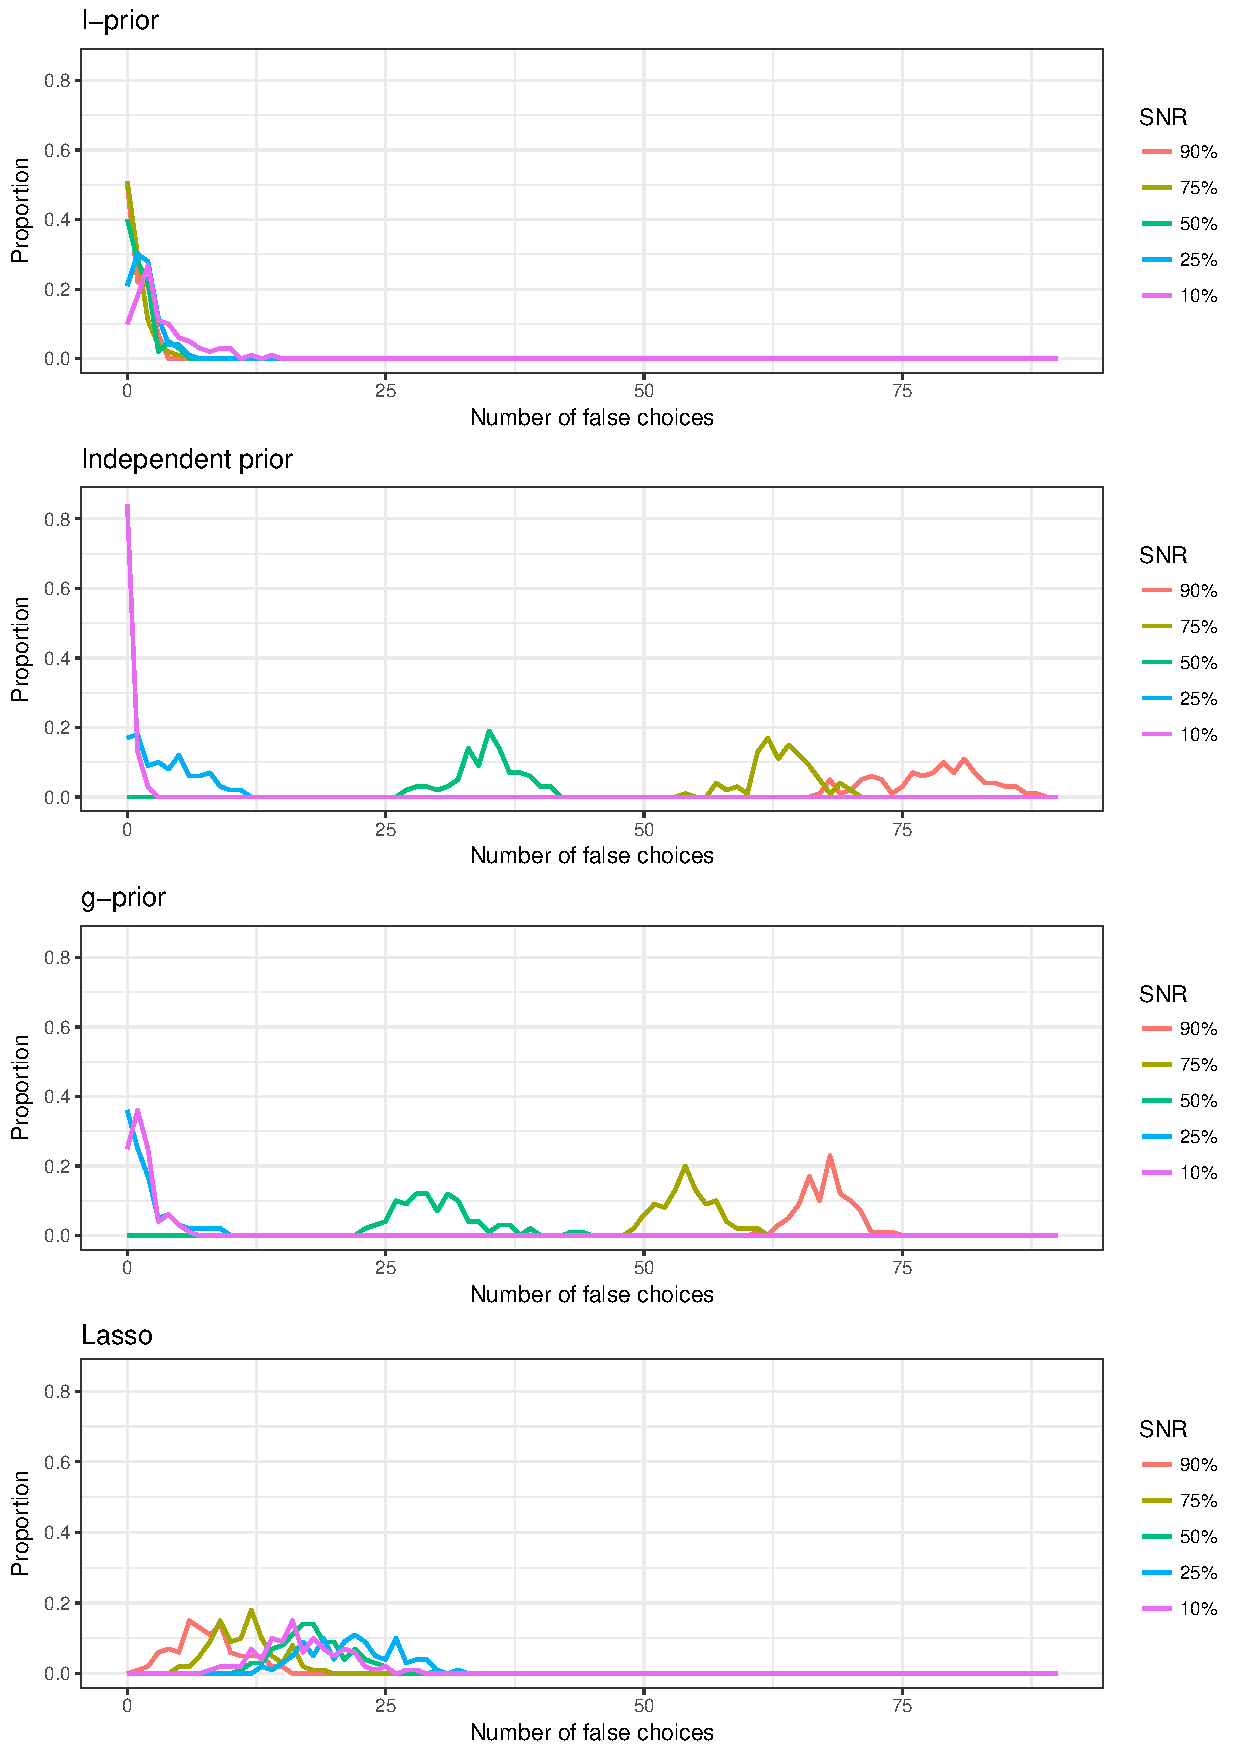
\includegraphics[width=0.991\textwidth]{figure/bvs_simres}
  \caption[Frequency polygons for the number of false choices]{Frequency polygons for the number of false choices for each of the four priors. The I-prior performs robustly well across the five scenarios tested, mostly yielding five or fewer false inclusions or exclusions. Spurious exclusions led to the independent and $g$-prior simultaneously performing well in low SNR and  badly in high SNR scenarios. The Lasso is known to be unreliable in the presence of collinearity.}
  \label{fig:simres}
\end{figure}

\index{Lasso}
The simulation results seem to indicate that the I-prior performs consistently well across all five scenarios, making no more than five false choices out of 100 (i.e. a 95\% correct selection rate) in at least 82\% of the time in the worst scenario.
We do not observe much difference between the $g$-prior and the independent prior, and while they behave poorly in high SNR scenarios, these two priors seem to perform extremely well in low SNR scenarios.
A high propensity to drop variables in these scenarios is a likely explanation, which does not necessarily indicate good performance---they perform well by contentiously omitting of a large number of unnecessary variables, especially in a two-stage procedure.
Finally, the Lasso is well known to yield poor selection performance under multicollinearity, so the results are expected.
The Lasso procedure was not subject to a two-stage approach because the Lasso does not provide information regarding posterior inclusion probabilities for individual variables.

We also inspect the sensitivity of the hyperprior choice of $\pi_j$ for the indicator variables on the number of false choices made.
\cref{fig:simres2} plots the mean number of false choices made in each of the five SNR scenarios with varying hyperprior setting for $\pi_j$.
From the plot, it is seen that for high SNR scenarios, setting $\pi_j$ too low increases the number of false exclusions.
Conversely, for low SNR scenarios, setting $\pi_j$ too high increases the number of false inclusions.
This makes sense: when the true model size is small, then setting $\pi_j$ too high encourages variables to be retained in the model, and vice versa.
While the optimal $\pi_j$ corresponds directly to the true SNR (e.g. SNR = 10\% performs best under $\pi_j=0.10$), \cref{fig:simres2} makes a case for $\pi_j=0.5$ to be a ``safe choice'' in the face of prior ignorance on model size.

\begin{figure}[hbt]
  \centering
  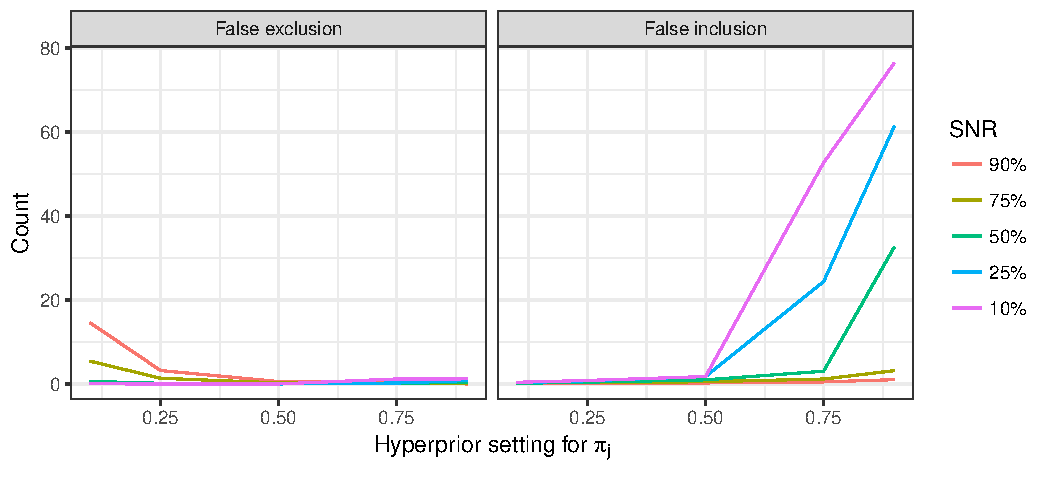
\includegraphics[width=0.95\textwidth]{figure/06-sens_analysis}
  \caption[Sensitivity analysis of hyperprior choice on number of false choices]{Average number of false choices (false inclusions or false exlusions) for the five different scenarios (SNR varied between 90\%, 75\%, 50\%, 25\% and 10\%) with different hyperprior settings for $\gamma_j\sim\Bern(\pi_j)$.}
  \label{fig:simres2}
\end{figure}
\vspace{-1em}

\section{Examples}

Now, we apply our I-prior Bayesian variable selection model to three real-world data sets that have all been previously analysed in the variable selection literature.
All examples were analysed in \proglang{R} using our \pkg{ipriorBVS} package \citep{jamil2018ripriorBVS} which contains a wrapper to \proglang{JAGS} \citep{plummer2003jags}.
Reproducible code is available at \url{http://myphdcode.haziqj.ml}.
In all analyses, a two-stage procedure was conducted for the I-prior model, where each stage consists of obtaining 15,000 MCMC samples (including 5,000 for burn-in).

\subsection{Aerobic data set}
\label{sec:aerobicbvs}
\index{aerobic data set}

\begin{figure}[htb]
	\centering
	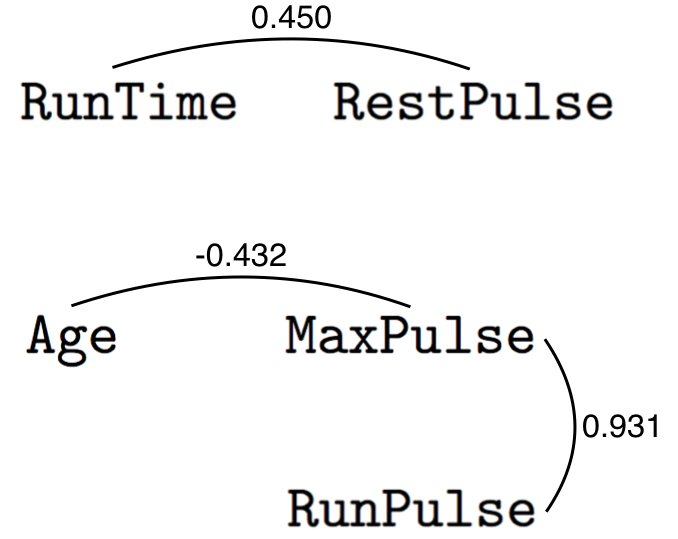
\includegraphics[height=1.3in]{figure/aerobic-cor}
	\caption[The sample correlations of interest in the aerobic fitness dataset]{The sample correlations of interest in the aerobic fitness dataset. These show variables with correlations greater than 0.4 in magnitude. \label{fig:aerobic-cor}}
\end{figure}

This dataset appeared in the \textit{SAS/STAT\textsuperscript{\textregistered} User's Guide} \citep{SAS2008} and was also analysed by \citet{Kuo1998}. 
It involves understanding the factors which affect aerobic fitness, which is measured by the ability to consume oxygen. 
A sample of $n=30$ male participants' had their physical fitness measured by means of simple exercise tests. 
The response variable contains measurement of oxygen uptake rate in mL/kg body weight per minute. 
The six covariates were the participants' age ($X_1$), weight ($X_2$), time taken to run one mile ($X_3$), resting heart rate ($X_4$), heart rate while running ($X_5$), and maximum heart rate during the exercise ($X_6$). 
This dataset, although small in size, is interesting to analyse because of the correlations between the variables, mainly due to the measurements being taken during the same exercise test. 
The sample correlations of interest are shown in \cref{fig:aerobic-cor}.

\begin{table}[htb]
\centering
\caption[Results for variable selection of the Aerobic data set]{Results for variable selection of the Aerobic data set. Note that the Bayes factors reported are the Bayes factors comparing any of the models to Model 1 (base model).}
\label{tab:aerobic}
\begin{tabular}{lrrrrrr}
\toprule
      &PIP    &Coef. (SD)  &Model 1 &Model 2 &Model 3 &Model 4 \\
\midrule
$X_1$ &0.685  &$-0.169 \ (0.14)$ &\cmark  &        &\cmark  & \\
$X_2$ &0.205  &$-0.017 \ (0.05)$ \\
$X_3$ &1.000  &$-0.745 \ (0.12)$ &\cmark  &\cmark  &\cmark  &\cmark \\
$X_4$ &0.168  &$-0.013 \ (0.05)$ \\
$X_5$ &0.663  &$-0.163 \ (0.15)$ &\cmark  &        &        &\cmark \\
$X_6$ &0.275  &$0.003  \ (0.10)$ \\
\midrule
      &&PMP   &0.564   &0.235   &0.105   &0.096 \\
      &&BF    &1.000   &0.418   &0.187   &0.170 \\
\bottomrule
\end{tabular}
\end{table}

Notice that \cref{tab:aerobic} reports only on four out of  $2^6 = 64$ possible models, but the sum of the posterior model probabilities add to one.
Naturally, models which are deemed important by virtue of data evidence are sampled more often, and in fact, models which are unpromising may not even get sampled.
So, MCMC methods does not need to list out all possible models because models which are never visited in the posterior state space are assigned a probability of zero.
The highest posterior model was found to be the model with the variables $X_1$, $X_3$ and $X_5$ (PMP = 0.564).
In \cref{fig:aerobic-densplot}, we can see that the point mass at zero overwhelms the rest of the values in the density plots for $X_2$, $X_4$ and $X_6$, and hence these variables were dropped.

\begin{figure}[H]
  \centering
  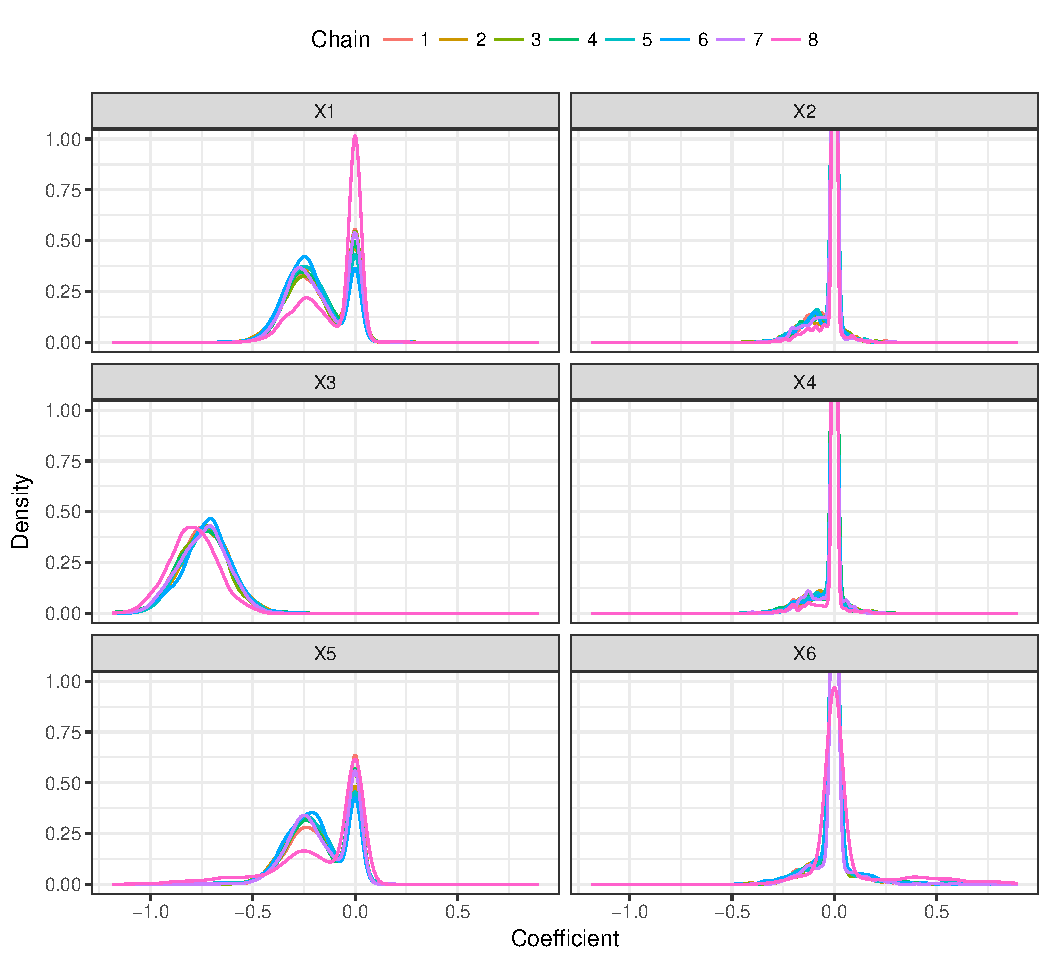
\includegraphics[width=\textwidth]{figure/06-aerobic_coef}
  \caption[Posterior density plots of the regression coefficients for the aerobic data set.]{Posterior density plots of the regression coefficients $\btheta$ for the aerobic data set. The spike at zero observed in the density plots for $X_2$, $X_4$ and $X_6$ is indicative of these variable being dropped often in the posterior samples.}
  \label{fig:aerobic-densplot}
\end{figure}

\subsection{Mortality and air pollution data}
\label{sec:airpollution}
\index{mortality and air pollution data set}

The next real world application comes from a paper by \citet{McDonald1973}. 
In it, the effects of air pollution on mortality in a US metropolitan area ($n=60$ and $p=15$) were studied. 
The response variable is the total age adjusted mortality rate, and the main pollution effects of interest were that of hydrocarbons (HC), oxides of nitrogen (NO\textsubscript{x}) and sulphur dioxide (SO\textsubscript{2}). 
Several other environmental and socioeconomic considerations were taken into account, otherwise the model may include unexplained variation caused by factors other than pollution. 
For example, a metropolitan area with a high proportion of the elderly should expect to have a higher mortality rate than one with a low proportion. 
All of the variables can be considered as continuous and real; \cref{tab:airpollution} provides a description of the variables.

\begin{table}[hbt]
\centering
\caption{Description of the air pollution data set.}
\label{tab:airpollution}
\begin{tabular}{ll}
\toprule
Variable                 & Description \\
\midrule
Mortality                & Total age adjusted mortality rate \\
Precipitation            & Mean annual precipitation (in) \\
Relative humidity        & Percent relative humidity, annual average at 1 p.m. \\
January temperature      & Mean January temperature ($^\circ$F) \\
July temperature         & Mean July temperature ($^\circ$F) \\
Population density       & Population per square mile in urbanised area \\
Household size & Population per household  \\
Education                & Median school years completed for those over 25 \\
Sound housing units      & Percentage of sound housing units (no defects) \\
Age >65 years            & Percent of population that is 65 years of age or over \\
Non-white                & Percent of urbanised area population that is non-white \\
White collar             & Percent employment in white-collar urbanised occupations \\
Income <\$3,000          & Percent of families with income under \$3,000 \\      
HC                       & Relative population potential of hydrocarbons \\     
NO\textsubscript{x}      & Relative population potential of oxides of nitrogen \\
SO\textsubscript{2}      & Relative population potential of sulphur dioxide \\       
\end{tabular}
\end{table}

\index{ridge regression}
\index{Mallows Cp@Mallow's $C_p$}
This dataset also contains several highly correlated variables which impedes a meaningful regression analysis. 
When the full model is fitted using ordinary least squares, none of the pollutant effects were found to be significant. 
Clearly, a variable selection method was required. 
\citet{McDonald1973} used a ridge regression technique to determine which variables to select and eliminate ``unstable'' coefficients found from a trace analysis. 
In addition, the authors also looked at a variable elimination method based on total squared error via Mallow's $C_p$.
The results are summarised in \cref{tab:poll}.

\begin{table}[htb]
\centering
\caption[Results for the mortality and air pollution BVS model.]{A comparison of the coefficient values obtained using ordinary least squares (full model), \citeauthor{McDonald1973}'s minimum $C_p$ and ridge analysis, and the I-prior. Standard errors/posterior standard deviations are given in parentheses. Values shaded grey indicate OLS regression coefficients not significant at the 10\% level.}
\label{tab:poll}
\begin{tabular}{lrrrr}
\toprule
& Full model & Min. $C_p$ & Ridge  & I-prior \\ \midrule
\emph{Environmental factors} \\
\hspace{0.5em} Precipitation            & 0.306 (0.14)                 & 0.247 (0.07)   & 0.230 (0.07)      & 0.254 (0.12)       \\
\hspace{0.5em} Relative humidity        & {\color{grymath} 0.009 (0.10)}  &                &                   &         \\
\hspace{0.5em} January temperature      & {\color{grymath} -0.318 (0.18)} & -0.164 (0.06)  & -0.172 (0.06)     & -0.195 (0.11)        \\
\hspace{0.5em} July temperature         & {\color{grymath} -0.237 (0.15)} & -0.073 (0.07)  &                   &         \\
\\
\emph{Demographic factors} \\
\hspace{0.5em} Population density       & {\color{grymath} 0.084 (0.09)}  &                & 0.091 (0.06)      &         \\
\hspace{0.5em} Household size & {\color{grymath} -0.232 (0.15)} &                &                   &         \\
\hspace{0.5em} Education                & {\color{grymath} -0.233 (0.16)} & -0.190 (0.06)  & -0.171 (0.07)     & -0.151 (0.12)        \\
\hspace{0.5em} Sound housing units   & {\color{grymath} -0.052 (0.15)} &                &                   &         \\
\hspace{0.5em} Age >65 years     & {\color{grymath} -0.213 (0.20)} &                &                   &         \\
\hspace{0.5em} Non-white             & 0.640 (0.19)                 & 0.481 (0.07)   & 0.462 (0.07)      &  0.517 (0.10)       \\
\hspace{0.5em} White collar          & {\color{grymath} -0.014 (0.12)} &                &                   &         \\
\hspace{0.5em} Income <\$3,000         & {\color{grymath} -0.009 (0.22)} &                &                   &         \\
\\
\emph{Pollution potential} \\
\hspace{0.5em} HC    & {\color{grymath} -0.979 (0.72)} &                &                   &         \\
\hspace{0.5em} NO\textsubscript{x} & {\color{grymath} 0.983 (0.75)}  &                &                   &         \\
\hspace{0.5em}  SO\textsubscript{2} & {\color{grymath} 0.090 (0.15)}  & 0.255 (0.06)   & 0.232 (0.06)      &  0.302 (0.09)        \\
\midrule
Size                     & 15                           & 6              & 6                 & 5         \\
$R^2$                    & 0.764                        & 0.541          & 0.553             & 0.676        \\ \bottomrule
\end{tabular}
\end{table}

In this case, the I-prior BVS model concurred with the overall finding of \citet{McDonald1973}, in that SO\textsubscript{2} was found to be a significant contributing factor towards mortality rates, while the rest of the pollutants were not.
the I-prior BVS model also obtained a model with the largest $R^2$ and the smallest size.
We note that the effect size for SO\textsubscript{2} is slightly larger under an I-prior, but generally, the rest of the I-prior coefficients are similar in magnitude and sign to the coefficients of the other two models.

\vspace{-0.5em}
\subsection{Ozone data set}
\label{sec:ozone}\index{ozone data set}
\vspace{-0.5em}
In this section, we replicate the Bayesian variable selection analysis of the Ozone dataset done by \citet[abbr. C\&M]{Casella2006} which appeared initially in \citet[abbr. B\&F]{Breiman1985}, and also show how Bayesian variable selection can help select important interaction terms. 
The data consists of daily ozone readings and various meteorological quantities, and the aim was to see which of these quantities contributed to the ozone concentration. 
The variables considered are explained in \cref{tab:ozone}. 

\begin{table}[htbp]
\centering
\caption[Description of the ozone data set]{Description of the ozone data set used in this analysis. The data is available from the \proglang{R} package \pkg{mlbench} \citep{mlbench}.}
\label{tab:ozone}
\begin{tabular}{ll}
\toprule
Variable     & Description \\
\midrule
$y$      & Daily maximum one-hour-average ozone reading (ppm) at Upland, CA \\
$X_1$    & Month: $1 = \text{January}, \dots, 12 = \text{December}$\\
$X_2$    & Day of month: $1,2,\dots$ \\
$X_3$    & Day of week: $1 = \text{Monday}, \dots, 7 = \text{Sunday}$ \\
$X_4$    & 500-millibar pressure height (m) measured at Vandenberg Air Force Base \\
$X_5$    & Wind speed (mph) at Los Angeles International Airport (LAX) \\
$X_6$    & Humidity (\%) at LAX \\
$X_7$    & Temperature ($^\circ$F) measured at Sandberg, CA \\
$X_8$    & Inversion base height (feet) at LAX \\
$X_9$    & Pressure gradient (mmHg) from LAX to Daggett, CA \\
$X_{10}$ & Visibility (mi) measured at LAX \\
$X_{11}$ & Temperature ($^\circ$F) measured at El Monte, CA \\      
$X_{12}$ & Inversion base temperature (degrees Fahrenheit) at LAX \\             
\end{tabular}

\end{table}

The data contains 366 points, one for each day of the leap year 1976. 
There are 163 data points containing missing data on some of the predictors, so we did a complete case analysis on the remaining 203 samples. 
Out of these 203, we randomly set aside 25 to use for validation, thus the $n$ used to train the model was $n=178$. 
The training and test set were repeated multiple times and results averaged in order to make a comparison to the unknown training and test set used in the other studies.
Out-of-sample prediction RMSE were obtained, as well as the coefficient of determination $R^2$.

C\&M removed the variables $X_{11}$ and $X_{12}$ before running their selection model, citing multicollinearity causing ill-conditioned design matrices. 
Upon inspection, there are indeed correlations among the variables as high as 0.93 for some of them, but not enough to cause rank deficiency in the design matrix and a degenerate $\XTX$ matrix.
The sample correlations $\widehat\Corr(X_7,X_{11}) =0.91$ and $\widehat\Corr(X_{11},X_{12}) = 0.93$ seemed to drive the decision to drop the two variables, and while it is a valid concern, we shall still conduct variable selection on the full set of 12 variables to see the performance of I-priors in the presence of multicollinearity in this real-world data set. 
On another note, the variables $X_1$, $X_2$ and $X_3$ were presumably intended to be categorical as in modelling seasonality in a time series data, but these were treated as continuous, as did C\&M. 
The results are compared in \cref{tab:ozoneres}.

\begin{table}[htb]
\centering
\caption{Results for variable selection of the Ozone data set using only linear predictors.}
\label{tab:ozoneres}
\begin{tabular}{llrrrr}
\toprule
Method                          &Variables            &Size &$R^2$ &RMSE \\
\midrule
I-prior                         &$X_1,X_6,X_{11}$     &3    &0.708 &0.554 \\
\citeauthor{Casella2006} (C\&M) &$X_6,X_7,X_8$        &3    &0.686 &0.992 \\
\citeauthor{Breiman1985} (B\&F) &$X_7,X_8,X_9,X_{10}$ &4    &0.669 &1.056 \\
\bottomrule
\end{tabular}
\end{table}

What we found was that the model selected using the I-prior does better in terms of $R^2$ as well as RMSE compared to the methods used by C\&M and B\&F. 
The average posterior model probability for $\{X_1,X_6,X_{11}\}$ as found by the I-prior was 0.722\footnotemark. 
One thing to note is that the I-prior model selected the variable $X_{11}$ instead of its highly correlated proxy $X_7$, which is what C\&M selected.
These two variables are temperature measurements at different locations in California.
As C\&M excluded $X_{11}$ from the model search it was of course never considered in their model selection process, and because we included it in ours, the variable selection model was able to consider both variables together and decide on the more appropriate one. 

\footnotetext{Since the total model space used was different between our method, C\&M and B\&F, it does not make sense to compare posterior model probabilities which we obtained. C\&M reported a model probability of 0.491 for their model, but this model was not selected at all using the I-prior.}

Interestingly, the distance as the crow flies between Sandberg, CA (location of temperature measurements for $X_7$) and Upland, CA (location of ozone readings) is roughly 121 km, but El Monte, CA (location of temperature measurements for $X_{11}$) is just 35 km away from Upland, CA.
It stands to reason that $X_{11}$ provides more geographical reliability than $X_7$.
Unless there is a strong insistence on deleting variables beforehand, we might not know for sure whether the variable was rightfully removed from consideration, as this example seems to prove.
Out of curiosity, running the variable selection model on the reduced variable space as C\&M did, we arrive at the same results as theirs.

\begin{figure}[htb]
  \centering
  \vspace{3pt}
  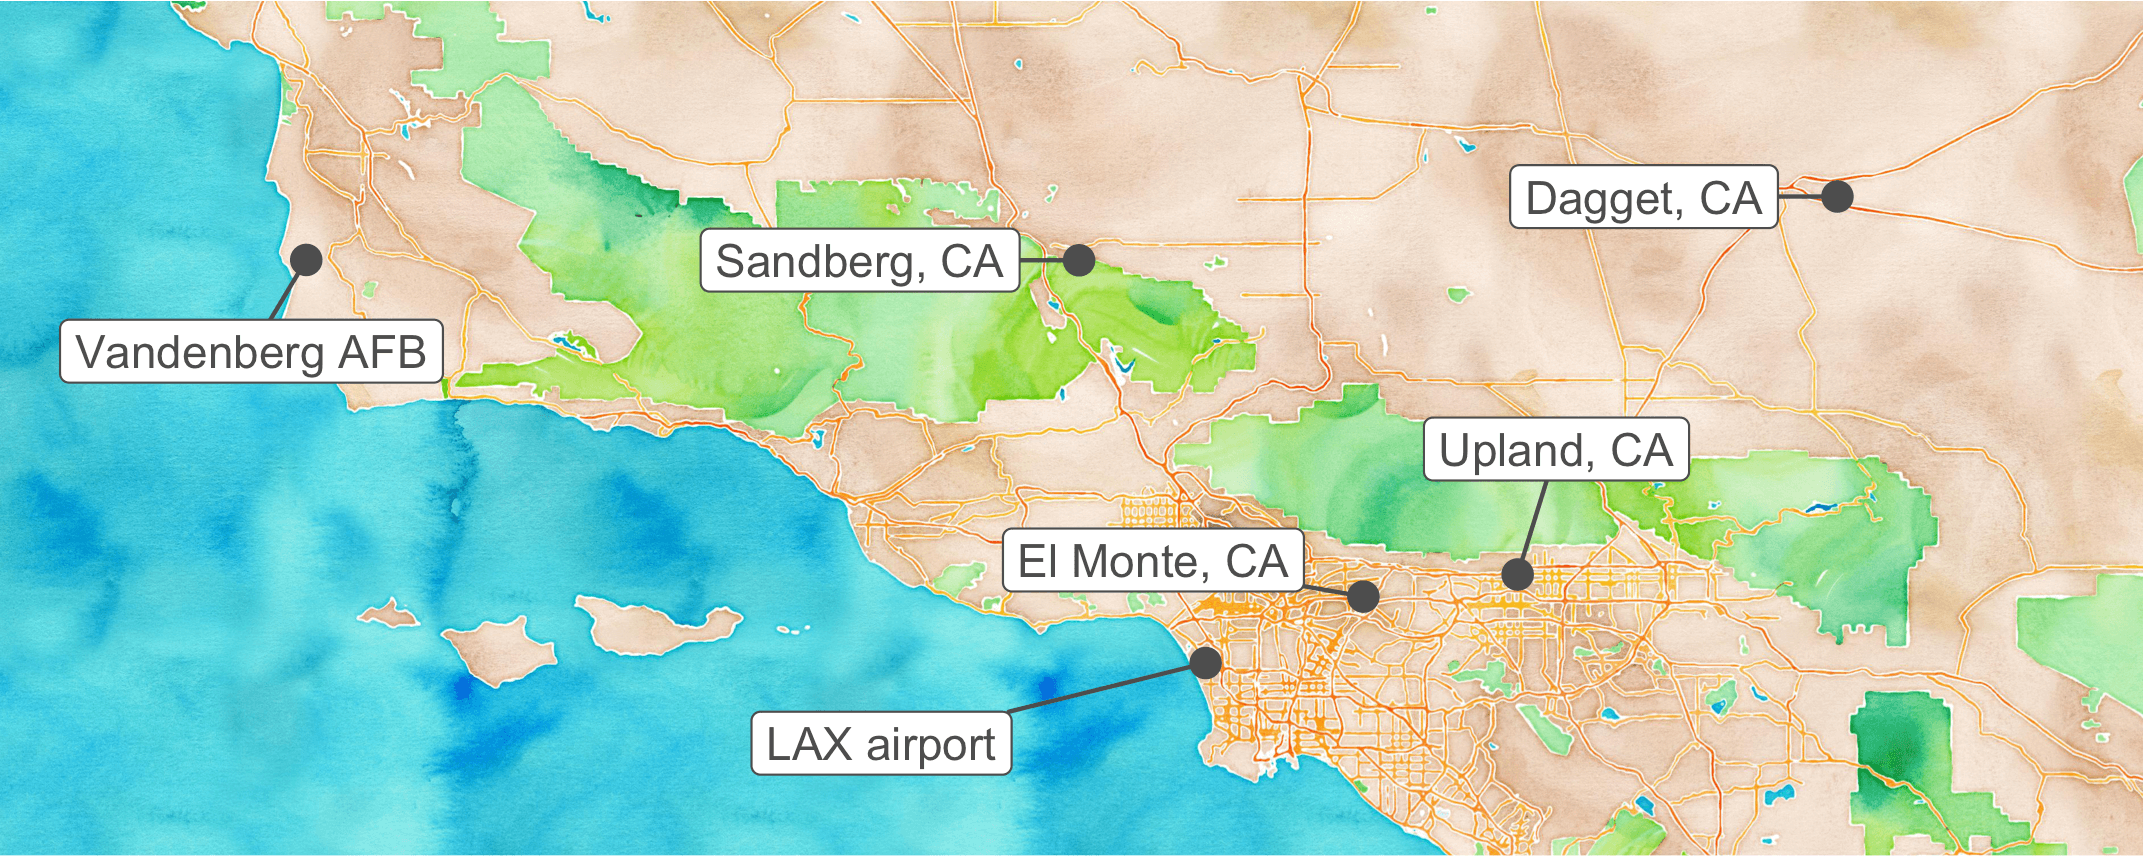
\includegraphics[width=\textwidth]{figure/06-ozone_map}
  \caption[Locations of the various points of interest in California, USA, related to the ozone measurements]{Locations\footnotemark~of the various points of interest in California, USA, related to the ozone measurements.}
  \label{fig:aerobic-densplot       }
\end{figure}
\footnotetext{Map tiles by \href{http://stamen.com/}{Stamen Design}, under \href{https://creativecommons.org/licenses/by/3.0/legalcode}{CC BY 3.0}. Data by \href{http://openstreetmap.org/}{OpenStreetMap}, under \href{https://creativecommons.org/licenses/by-sa/3.0/legalcode}{CC BY-SA 3.0}. Created using the \pkg{ggmap} package \citep{ggmap} in \proglang{R}.}

\index{interaction}
We then used the I-prior method to select between the squared terms and all level two interactions, in addition to all the variables, in an effort to improve model prediction. 
For 12 such variables, the number of variables to select becomes $12 + 12 + 12(12 - 1)/2 = 90$. 
By doing so, we were able to improve the model to give a slightly better predictive ability.
The results are shown below in \cref{tab:resozone2}. 
The I-prior again selected a model which was superior in terms of $R^2$ and RMSE compared to that obtained by C\&M.

\begin{table}[htb]
\centering
\caption{Results for variable selection of the Ozone data set using linear, squared and two-way interaction terms.}
\label{tab:resozone2}
\begin{tabular}{llrrrr}
\toprule
Method                          &Variables            &Size &$R^2$ &RMSE \\
\midrule
I-prior                         
&{\footnotesize $X_1,X_5,X_6,X_{11},X_{12},X_1^2,X_9^2,X_6X_{11},X_6X_{12},X_7X_9$}     
&10    &0.812 &0.503 \\
C\&M
&{\footnotesize $X_2,X_1^2,X_7^2,X_9^2,X_1X_5,X_2X_6,X_3X_7,X_4X_6,X_6X_8,X_6X_{10}$}   &10    &0.758 &0.873 \\
\bottomrule
\end{tabular}
\end{table}

\section{Conclusion}

The model selection problem is an important one in statistics, but highly contentious.
\citet{miller2002subset} writes that many statisticians view model selection as ``unclean'' or ``distasteful'', and that ``terms such as `fishing expeditions', `torturing the data until they confess', `data mining', and others are used as descriptions of these practices''. 
The disagreement with the principle of model selection stems from the belief in the mantra that models should only be built by thoughtfully choosing variables which are expected to influence the response by appealing to substantive theory, and not by virtue of optimising some model selection criterion.
However, variable selection as an exploratory study is certainly justified by many practical applications, especially when there is a genuine desire to know the most reasonable, parsimonious and interpretable model.
Through variable selection exercises, we can learn which covariates are important, and which are negligible, in explaining the variation in the response.
%arguably variable selection from a prescreening as part of data cleanup to remove problematic variables, such as those inducing a high degree of collinearity. how do we know we are deleting the correct variable?

The Bayesian variable selection method that we have seen has the appeal of reducing the problem of model search into one of estimation. 
At the outset, we aimed to seek a model which: 1) requires little tuning on the part of the user; 2) would work well in the presence of multicollinearity; and 3) is able to work well with little to no prior information. 
The I-prior on the regression coefficients in \citeauthor{Kuo1998}'s  \citeyearpar{Kuo1998} spike-and-slab stochastic search framework achieves this aim.

The attractive feature of a Bayesian approach to variable selection is the ability to simultaneously shrink and select predictors, thereby incorporating model uncertainty in the regressors.
Sparsification is not ``hard coded'', in the sense that regression coefficients are assigned a value of zero with some positive probability in the posterior.
This is unlike the regularisation or penalised log-likelihood approach to variable selection using the Lasso, elastic net, and so on, whereby sparsity is induced at the mode, but not in the posterior distribution \citep{scott2014predicting}.
This translates to being provided with a single variable selection decision, rather than information that is coded through a probability distribution.

We discuss three areas to concentrate on for future research and improvement:
\begin{enumerate}
  \item \textbf{\boldmath$p>n$ cases}. 
  Typically, when there is insufficient information in the data to inform the estimation, then additional information is sought from the priors. 
  In our case, the I-prior covariance involves the inverse of a low rank matrix which is not invertible.
  A $p$-variate normal distribution with a singular covariance matrix will only have a probability distribution defined on a low dimensional subspace.
  The issue may however be computational---it might be worth exploring the generalised inverse, or study ways in which to avoid the inverse computation in the Gibbs sampler.
  As a matter of fact, we note that the posterior precision for $\bbeta$ can be written as 
  \begin{align*}
    \tilde \bB^{-1}
    &= \big(\bX_\gamma^\top \bX_\gamma + (\kappa \XTX)^{-1}\big)^{-1} \\
    &= \bX_\gamma^\top \bX_\gamma \big((\bX_\gamma^\top \bX_\gamma)^2 + \kappa \bI_p \big)^{-1}
  \end{align*}
  which avoids the need for inverting the low-rank matrix $\bX_\gamma^\top \bX_\gamma$.
  
  \item \textbf{Improvement in computational time}. 
  Although the model itself is not computationally intensive to run (roughly $O(np^2)$ in time per Gibbs iteration), the main bottleneck is the reliance on a stochastic sampling algorithm.
  As in the previous chapter, variational inference is a promising area to look into, especially given that the Gibbs conditional distributions were straightforward to obtain, and these might be similar to a mean-field variational distribution.
  If this is successful, then it is expected to reduce computational time and avoid convergence issues that comes with traditional MCMCs.
  Variational inference with spike-and-slab priors on regression coefficients was studied by \citet{ormerod2017variational}.
  
  \item \textbf{Extension to generalised linear models}.
  \citet{Kuo1998} in their paper already provided a sketch of how the variable selection model would work.
  With the ideas in \cref{chapter5}, we can extend the I-prior variable selection to categorical responses when the continuous latent propensities are modelled using linear functions.
  Such an approach has been implemented in gene selection studies, for which the variables are gene expressions and the responses are presence of a particular disease \citep{lee2003gene}.
\end{enumerate}

Finally, it should be mentioned that more complex variable selection models can be coded with the $\gamma$ indicators.
For instance, in selecting squared or interaction terms, we can insist on having the model select the main term if the squared or interaction term is selected:
\[
  y_i = \alpha + \gamma_1 \beta_1 x_{1i} + \gamma_2 \beta_2 x_{2i} + \gamma_1 \gamma_2\gamma_3 \beta_3 x_{1i}x_{2i}.
\]
Or perhaps, we could use a single $\gamma$ indicator for the dummy variables which make up a single categorical covariate, which we would then infer on the selection of the single covariate rather than each individual category of the covariate.

\hClosingStuffStandalone
\end{document}